%%%%%%%%%%%%%%%%%%%%%%%%%%%%%%%%%%%%%%%%%%%%%%%%%%%%%%%%%%%%%%%%%%%%%%%%%%%%%%%%
\section{Discussion and Research Gaps}
\label{sec:discussion}
%%%%%%%%%%%%%%%%%%%%%%%%%%%%%%%%%%%%%%%%%%%%%%%%%%%%%%%%%%%%%%%%%%%%%%%%%%%%%%%%

The results of this systematic review show that \gls{dectnr} has developed
rapidly from an \gls{imt2020} candidate technology into an active research
platform for decentralized and industrial wireless communication. The
literature now spans PHY and MAC operation, multi-hop networking, reliability,
resource management, energy efficiency, positioning, coexistence, and
application-oriented implementations. However, the evidence is unevenly
distributed across these areas and remains heterogeneous in both methodology
and experimental scale. This section interprets the quantitative and technical
findings of the review, identifies the principal limitations of the current
evidence base, and derives research priorities for the continued development of
DECT NR+.

%%%%%%%%%%%%%%%%%%%%%%%%%%%%%%%%%%%%%%%%%%%%%%%%%%%%%%%%%%%%%%%%%%%%%%%%%%%%%%%%
\subsection{Maturity of the DECT-2020 NR Research Landscape}
\label{subsec:research_maturity}
%%%%%%%%%%%%%%%%%%%%%%%%%%%%%%%%%%%%%%%%%%%%%%%%%%%%%%%%%%%%%%%%%%%%%%%%%%%%%%%%

The publication trend indicates a rapidly expanding but still comparatively
young research field. Approximately 75\% of the 51 included studies were
published between 2024 and July 2026, and 36 studies appeared as conference
publications. This concentration of recent work suggests that the research
community is still actively exploring fundamental mechanisms, implementation
strategies, and application opportunities rather than converging on mature and
widely validated design practices.

Research maturity also differs substantially across technical areas. PHY, MAC,
and routing/mesh networking are the most frequently investigated topics, with
22, 22, and 23 studies addressing these areas, respectively. Experimental,
testbed, or application-related aspects appear in 18 studies, indicating a
growing transition from analytical feasibility toward implementation. In
contrast, scheduling and resource allocation, positioning, security,
coexistence, and multi-RAT integration remain less extensively investigated.
The current evidence base is therefore strongest for the fundamental
communication mechanisms and weaker for several functions that become
increasingly important when DECT NR+ is deployed as part of a complete
industrial communication system.

The methodological distribution reinforces this interpretation. Simulation is
used in 32 studies and analytical or modeling approaches in 23, whereas 16
studies employ experimental or testbed evaluation. Hardware-based investigations
are particularly important because they expose implementation effects that are
difficult to represent completely in abstract models, including industrial
propagation, modem energy consumption, implementation-dependent throughput,
gateway processing, and RX--TX turnaround behavior
\cite{wassmannPerformanceDECT2020NR2024,
bandaraExperimentalValidationAnalysis2025,
grafWhatExpectWhen2026,
piresDECT2020NREnergy2026b,
alizaiMeasurementDrivenLatencyAnalysis2026}.
Consequently, the literature demonstrates that DECT NR+ has moved beyond
proof-of-concept evaluation, but experimental maturity has not yet reached the
same level across all research areas.

%%%%%%%%%%%%%%%%%%%%%%%%%%%%%%%%%%%%%%%%%%%%%%%%%%%%%%%%%%%%%%%%%%%%%%%%%%%%%%%%
\subsection{Cross-Layer and Application-Oriented Design}
\label{subsec:cross_layer_gaps}
%%%%%%%%%%%%%%%%%%%%%%%%%%%%%%%%%%%%%%%%%%%%%%%%%%%%%%%%%%%%%%%%%%%%%%%%%%%%%%%%

One of the clearest conclusions of the technical synthesis is that DECT NR+
performance is inherently cross-layer. PHY configuration affects data rate,
coverage, reliability, airtime, and energy consumption
\cite{grafParetoOptimalityApproach2026a}; MAC and channel-access mechanisms
influence contention and access delay
\cite{samuylovPerformanceMACLayer2024a,
gaidamakaOptimizingDelaysRandom2025}; and routing decisions affect hop count,
forwarding load, latency, and reliability
\cite{asifURLLCBasedMultiHopCommunication2025,
alamDLRoutingPerformance2026a,
rauwolfTopologyAwareDeepReinforcement2026a}. Network lifetime is additionally
affected by router availability and role assignment
\cite{nihtilaEnergyConsumptionDECT20202022,
nihtilaEnergySavingRouter2022}, while hardware constraints can alter the
latency achievable by otherwise efficient schedules
\cite{alizaiMeasurementDrivenLatencyAnalysis2026}.

Figure~\ref{fig:cross_layer_framework} summarizes these dependencies from an
application-oriented perspective. Industrial service requirements are
translated through scheduling and QoS management, MAC and channel access,
routing and mesh networking, PHY configuration, and finally the capabilities
and constraints of the hardware implementation. At the same time, traffic
characteristics, propagation conditions, topology, and device capabilities
influence several layers simultaneously. The resulting application-level
performance is therefore determined by interactions across the protocol stack
rather than by any individual mechanism in isolation.

\begin{figure*}[t]
    \centering
    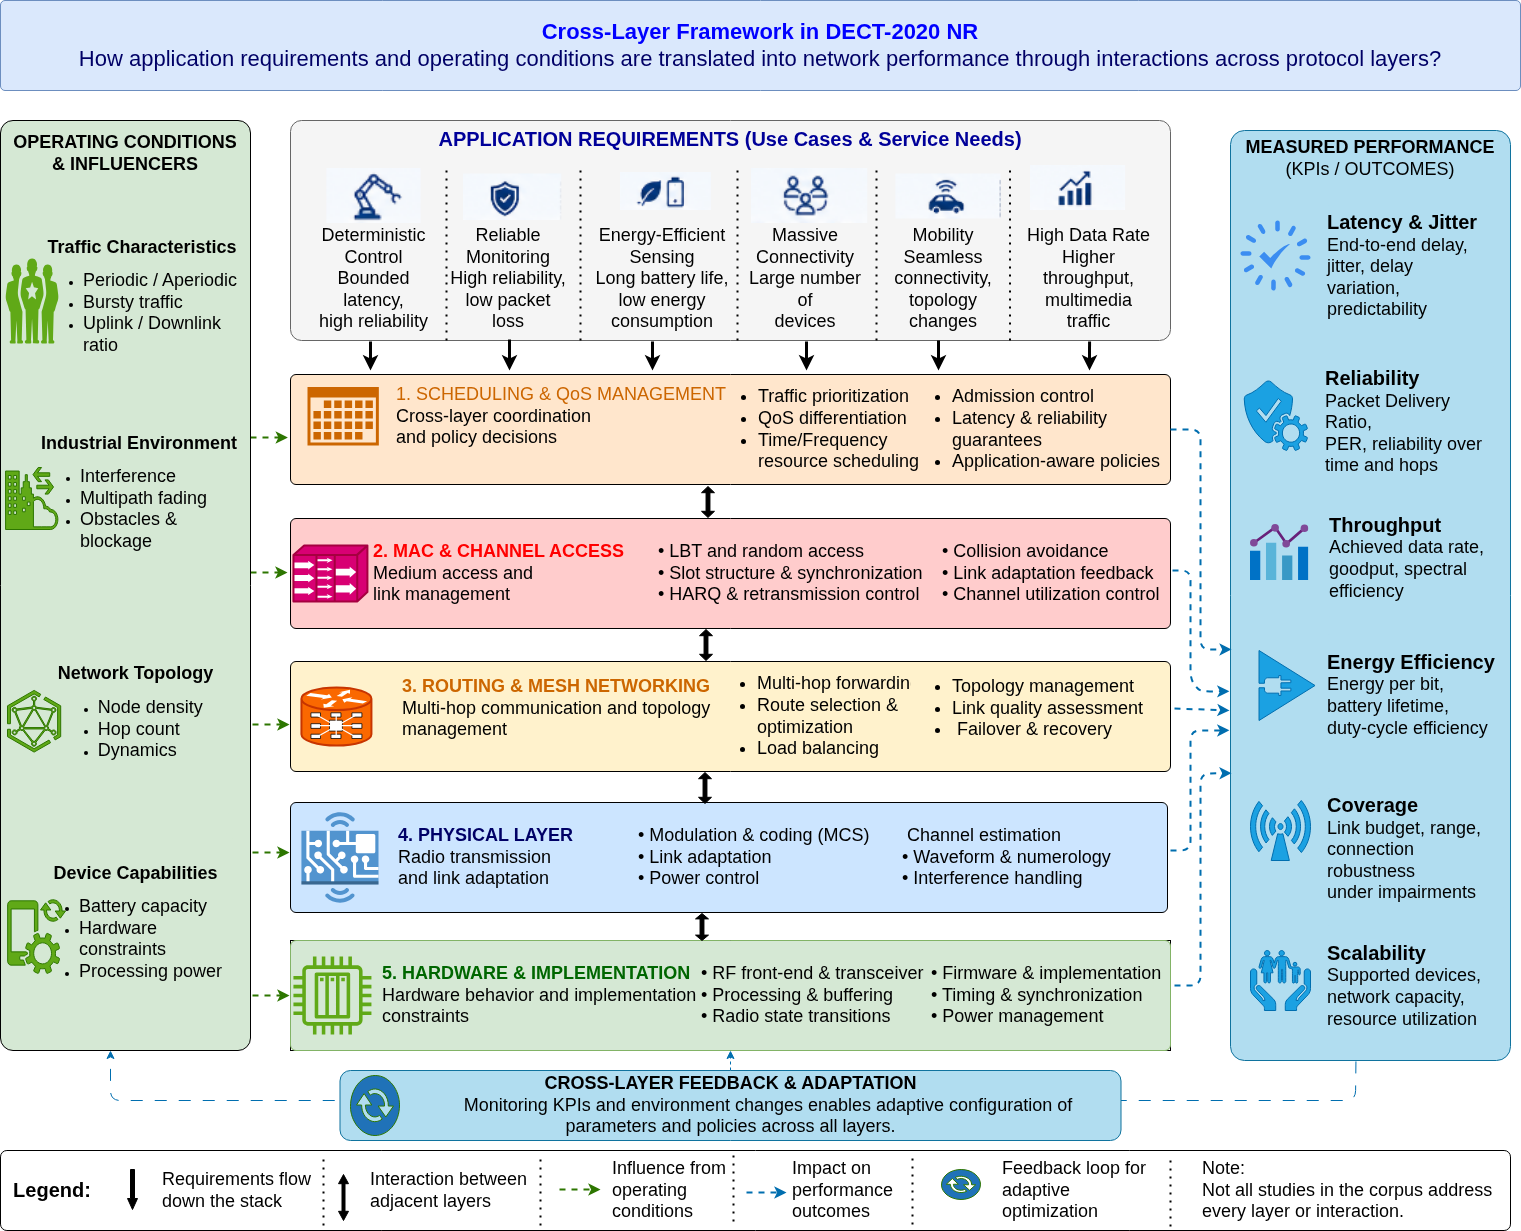
\includegraphics[width=\textwidth]{figures/CrossLayerFramework.png}
    \caption{Application-oriented cross-layer framework for DECT-2020 NR,
    illustrating how application requirements and operating conditions interact
    with scheduling, MAC, routing, PHY, and hardware mechanisms to determine
    measurable application-level performance.}
    \label{fig:cross_layer_framework}
\end{figure*}

This interaction is especially important for industrial applications because
their requirements differ substantially. Periodic sensing may prioritize
energy efficiency and long device lifetime, deterministic control requires
bounded latency and high reliability, mobile systems introduce topology and
routing dynamics, and professional media applications combine stringent timing
with sustained traffic. Existing implementations demonstrate the feasibility
of several such application classes
\cite{mudriievskyiCHEAP5GDECT2024a,
poetsProfessionalNetworkedAudio2025,
piresDECT2020NREnergy2026b}, but the literature does not yet provide a
systematic mapping from application requirements to complete PHY, MAC,
scheduling, routing, and energy-management configurations.

This gap is particularly visible in scheduling and resource allocation.
Although DECT NR+ provides flexible resource assignment and decentralized
channel access, comparatively few studies treat application-aware scheduling
as their primary problem. Existing work demonstrates benefits from adaptive
random access, resource configuration, and application-dependent PHY selection
\cite{gaidamakaOptimizingDelaysRandom2025,
glazkovImprovingNearURLLCServices2025,
grafParetoOptimalityApproach2026a}, but the joint management of deterministic,
reliability-oriented, high-throughput, and energy-constrained traffic remains
insufficiently explored. Future work should therefore move from isolated
parameter optimization toward configurable cross-layer strategies that select
operating points according to explicit application requirements and observed
network conditions.

%%%%%%%%%%%%%%%%%%%%%%%%%%%%%%%%%%%%%%%%%%%%%%%%%%%%%%%%%%%%%%%%%%%%%%%%%%%%%%%%
\subsection{Experimental and Methodological Gaps}
\label{subsec:experimental_gaps}
%%%%%%%%%%%%%%%%%%%%%%%%%%%%%%%%%%%%%%%%%%%%%%%%%%%%%%%%%%%%%%%%%%%%%%%%%%%%%%%%

A second major limitation concerns the gap between the scale and abstraction of
simulation studies and the conditions evaluated experimentally. Analytical and
system-level studies frequently consider dense and multi-hop deployments,
whereas physical experiments typically involve smaller device populations,
point-to-point communication, or relatively simple static topologies. Recent
multi-hop and application-oriented prototypes represent important progress
\cite{piresDECT2020NREnergy2026b,
poetsProfessionalNetworkedAudio2025}, but large physical deployments combining
routing, scheduling, heterogeneous traffic, mobility, and interference remain
rare.

This distinction matters because physical implementations introduce effects
that are commonly simplified or omitted in simulation. Radio-state
transitions, processing and buffering delays, firmware behavior,
synchronization, gateway processing, and transceiver turnaround can contribute
directly to application-visible performance
\cite{bandaraExperimentalValidationAnalysis2025,
piresDECT2020NREnergy2026b,
alizaiMeasurementDrivenLatencyAnalysis2026}. Protocol-level improvements
should therefore increasingly be evaluated together with the implementation
constraints of the target hardware.

Comparison across experimental studies is further complicated by the absence
of common benchmark configurations. Payload size, MCS, transmit power, traffic
load, topology, channel conditions, measurement duration, hardware platform,
and even the boundaries used to define latency differ between studies.
Consequently, apparently different performance results may reflect different
experimental conditions rather than differences in the mechanisms being
evaluated. A reproducible DECT NR+ evaluation framework should therefore report
at least the PHY configuration, channel and bandwidth, transmit power, packet
size, traffic model and offered load, number of devices, topology and hop
count, interference conditions, firmware or modem version, and measurement
duration.

The reported \glspl{kpi} also reveal an imbalance in the current evidence.
Packet loss and PER are widely evaluated, whereas application-level metrics
such as jitter, localization error, AoI, fairness, and connection density are
reported much less frequently. For latency-sensitive industrial systems,
average delay alone is insufficient because rare but large delays may determine
whether application deadlines are satisfied. Future evaluations should
therefore increasingly report latency distributions and high percentiles
together with reliability, jitter, energy consumption, and application-specific
performance measures.

Long-duration and failure-oriented validation is another important gap.
Industrial networks must continue operating under interference, node failures,
route changes, mobility, bursty traffic, and changing propagation conditions.
Experiments lasting hours or days, together with controlled fault injection and
recovery analysis, would provide stronger evidence of deployment readiness than
short measurements under nominal conditions.

%%%%%%%%%%%%%%%%%%%%%%%%%%%%%%%%%%%%%%%%%%%%%%%%%%%%%%%%%%%%%%%%%%%%%%%%%%%%%%%%
\subsection{Research Gaps and Future Research Priorities}
\label{subsec:future_directions}
%%%%%%%%%%%%%%%%%%%%%%%%%%%%%%%%%%%%%%%%%%%%%%%%%%%%%%%%%%%%%%%%%%%%%%%%%%%%%%%%

The preceding analysis indicates that the next phase of DECT NR+ research
should focus less on demonstrating individual mechanisms in isolation and more
on validating how those mechanisms interact within complete industrial
systems. Table~\ref{tab:research_gaps} consolidates the principal gaps
identified across the review and maps them to corresponding research
priorities.

\begin{table*}[t]
\centering
\caption{Key research gaps and future research priorities for DECT-2020 NR.}
\label{tab:research_gaps}
\renewcommand{\arraystretch}{1.12}
\small
\begin{tabular}{p{3.0cm} p{5.3cm} p{7.0cm}}
\hline
\textbf{Research Area} &
\textbf{Identified Gap} &
\textbf{Future Research Priority} \\
\hline

Cross-layer and application-oriented design &
PHY, MAC, scheduling, routing, and energy mechanisms are predominantly
investigated separately, with limited mapping from application requirements to
complete network configurations. &
Develop cross-layer configuration methods that translate latency, reliability,
traffic, mobility, density, and energy requirements into coordinated protocol
and radio parameters. \\

Scheduling and resource allocation &
Application-aware scheduling under heterogeneous traffic and competing
\gls{qos} requirements remains comparatively underexplored. &
Develop deterministic and reliability-oriented scheduling and resource
allocation for coexisting periodic, event-driven, bursty, and
energy-constrained traffic. \\

Large-scale mesh networking &
Large and dense networks are primarily evaluated analytically or through
simulation, while physical multi-hop testbeds remain comparatively small. &
Validate routing, topology management, scalability, mobility, congestion, and
recovery using larger hardware deployments under realistic traffic and
interference. \\

Experimental methodology &
Experimental configurations, measurement boundaries, hardware platforms, and
reported \glspl{kpi} vary substantially across studies. &
Establish reproducible benchmark scenarios and standardized reporting of radio,
traffic, topology, hardware, firmware, interference, and measurement
conditions. \\

Reliability and deterministic communication &
Latency and reliability are widely investigated, but tail behavior,
predictability, failures, and sustained operation receive less attention. &
Evaluate latency distributions, deadline satisfaction, reliability, and
recovery under interference, topology changes, retransmissions, failures, and
long-duration workloads. \\

Energy-aware networking &
Energy is frequently evaluated separately from routing, reliability, latency,
and network availability. &
Jointly investigate PHY adaptation, sleep scheduling, router-role management,
routing, residual energy, and application \gls{qos} to optimize network
lifetime. \\

Positioning and localization &
Positioning has received substantially less experimental attention than core
communication mechanisms. &
Validate integrated communication and positioning under industrial
propagation, mobility, NLoS conditions, and realistic anchor deployments. \\

Security, coexistence, and heterogeneous integration &
DECT NR+-specific security, coexistence, and multi-RAT operation remain
comparatively immature. &
Investigate secure multi-hop operation, authentication, interference-aware
coexistence, failover, and integration with Wi-Fi, cellular, and industrial
networks. \\

Hardware-aware system design &
Radio turnaround, processing, buffering, firmware, and other
implementation-specific effects are not consistently represented in system
models. &
Integrate hardware constraints into latency, scheduling, energy, and
cross-layer models and validate the resulting designs experimentally. \\

\hline
\end{tabular}
\end{table*}

Several priorities cut across the individual areas in
Table~\ref{tab:research_gaps}. Multi-objective configuration is required
because improvements in latency, reliability, throughput, and energy can
conflict \cite{grafParetoOptimalityApproach2026a}. Reliability-oriented
mechanisms should increasingly be validated under mixed traffic and changing
network conditions
\cite{samuylovEmpoweringNearURLLCIoT2025,
glazkovImprovingNearURLLCServices2025,
ahmadMACLayerProtocolUltraReliable2025}, while energy-aware networking should
combine router management, sleep behavior, routing, and radio configuration
rather than treating transmit power in isolation
\cite{nihtilaEnergyConsumptionDECT20202022,
nihtilaEnergySavingRouter2022,
grafParetoOptimalityApproach2026a}.

Less mature areas also require broader experimental attention. Positioning
results demonstrate the potential for communication-assisted localization
\cite{saikkoPositioningDECT2020NR2024,
saikkoPositioningTrackingDECT20202025}, and recent security and heterogeneous
networking studies show that DECT NR+ can be integrated with wider network
infrastructures
\cite{ngoIoTDeviceAuthentication2025,
dangEWDCIntegratingDECT20202025a,
dangUniRATUnifiedDECT20202026}. These directions now require evaluation under
realistic industrial mobility, interference, security, and failover
conditions.

Overall, the principal challenge is no longer only to demonstrate that
individual DECT NR+ mechanisms can achieve favorable performance, but to
determine how they should be configured and combined to provide predictable
application-level behavior under realistic scale, traffic, topology,
interference, energy, and hardware constraints. Addressing this challenge
through reproducible and increasingly large-scale experimental evaluation will
be essential for translating the flexibility of DECT NR+ into dependable
industrial wireless systems.